\chapter{Results and Discussion}
\label{chap:results_discussion}

\section{Iloilo Road Network Representation}
\label{chap:iloilo_representation}

The final network was rendered using OSMnx and Matplotlib, as shown in Figure 5.1. The graph captures the connectivity of the districts, including the complex bridging segments between Mandurriao and the City Proper that is based on the DPWH Atlas of Iloilo 2024.

\begin{figure}[ht]
    \centering
    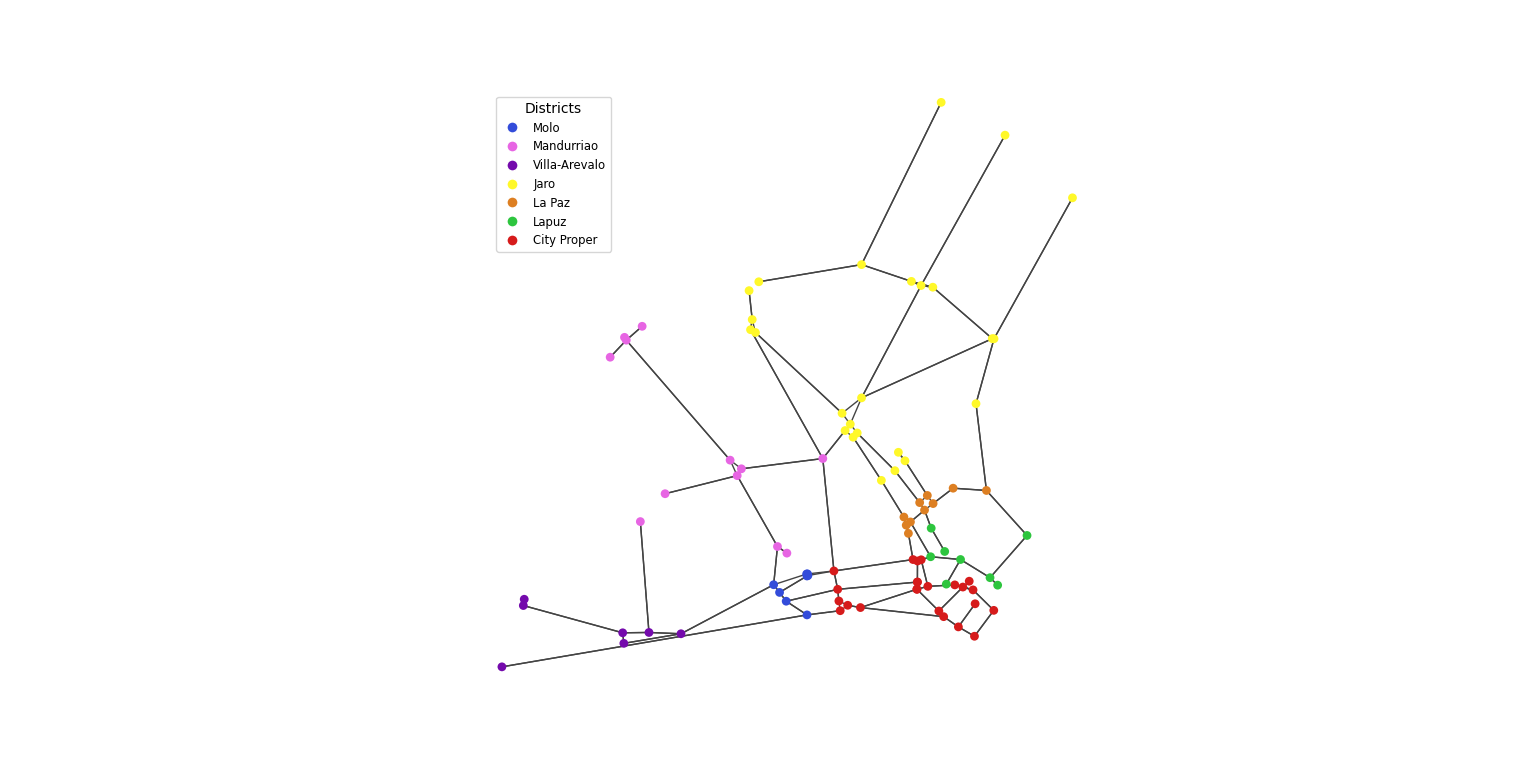
\includegraphics[width=\textwidth, height=7cm]{figures/figure-4.png}
    \caption{Iloilo City Directed Graph} 
    \label{fig:network_map}
\end{figure}

% \begin{table}[H]
%     \centering
%     \label{tab:network_stats}
%     \begin{tabular}{|l|c|}
%         \hline
%         \textbf{Metric} & \textbf{Value} \\ \hline
%         Total Number of Nodes (Intersections) & 92 \\ \hline
%         Total Number of Directed Edges (Road Segments) & 218 \\ \hline
%     \end{tabular}
%         \caption{Total Number of Nodes and Directed Edges of the Unified Iloilo City Network}
% \end{table}

% Table \ref{fig:network_map} Shows the total number of nodes and directed edges in the unified network. Here, the total number of nodes are 82 while the total number of directed edges are 218.

\section{Theoretical Topological Baseline}
\label{chap:topological_baseline}

Results show that there is an existence of possible Braess’s Paradox links within the Iloilo City network. Across the simulated permutations, the algorithm identified 8289 distinct Origin-Destination routing scenarios where the removal or directional restriction of a road mathematically improved Total System Travel Time (TSTT) within the model. Specifically, 4627 of these candidate links were unidirectional closures, while 3662 links were found in bidirectional closures. The severity of these inefficiencies is substantial, with the maximum record PoA being 1.5815. These metrics indicate that under specific volume thresholds, uncoordinated selfish routing performs 58,15\% worse than system optimal routing, suggesting that the current physical topology allows for counterintuitive shortcuts.

\subsection{Analysis of Network Inefficiencies and Price of Anarchy (PoA)}
\label{sec:network_inefficiencies_PoA}

Different traffic management policies can lead to a variety of dynamic outcomes, thus, the researchers categorized the most significant instances of the Braess Paradox by closure type to better illustrait their implications.

\subsection{Unidirectional Road Closures}
\label{sec:unidirectional_closures}

Table~\ref{tab:5.1a} shows the top segments where unidirectional closures yielded the highest frequencies of roads closed that improved the system when removed. On the other hand, Table~\ref{tab:5.2a} highlights the routing scenarios where the PoA was maximized, and the road closure caused improvement to the travel time

\begin{table}[htbp]
    \centering
    \renewcommand{\thetable}{5.1a}

    \begin{tabular}{|l|l|l|c|c|}
    \hline
    \textbf{Road Name} & \textbf{From} & \textbf{To} & \textbf{Frequency} & \textbf{Max PoA} \\ \hline
    Gen Luna St 3 (Rev) & Proper - 9 & Proper - 8 & 271 & 1.5815 \\ \hline
    Gen Luna St 3 & Proper - 8 & Proper - 9 & 210 & 1.5150 \\ \hline
    Gen Luna St 2 (Rev) & Proper - 8 & Proper - 7 & 159 & 1.3886 \\ \hline
    Gen Luna St 2 & Proper - 7 & Proper - 8 & 143 & 1.3611 \\ \hline
    Huervana St - Rizal St & Lapaz - 1 & Lapaz - 2 & 137 & 1.4747 \\ \hline
    \end{tabular}
    \caption{}
    \label{tab:5.1a}
\end{table}

{
\small 
\setlength{\tabcolsep}{3pt} 
\renewcommand{\thetable}{5.2a}
\begin{longtable}{|p{2.5cm}|p{1.5cm}|p{1.6cm}|p{1.2cm}|p{1.4cm}|p{1.4cm}|p{1.4cm}|p{1.3cm}|p{1.3cm}|} 

\hline
\textbf{Road Name} & \textbf{Origin of Trip} & \textbf{Dest. of Trip} & \textbf{Max PoA} & \textbf{Crit. Vol.} & \textbf{Base. TSTT} & \textbf{New TSTT} & \textbf{Time Saved} & \textbf{Avg. Saved} \\ \hline
\endfirsthead

\hline
\textbf{Road Name} & \textbf{Origin of Trip} & \textbf{Dest. of Trip} & \textbf{Max PoA} & \textbf{Crit. Vol.} & \textbf{Base. TSTT} & \textbf{New TSTT} & \textbf{Time Saved} & \textbf{Avg. Saved} \\ \hline
\endhead

\hline
\endfoot

\hline
\caption{}
\label{tab:5.2a}
\endlastfoot

Gen Luna St 3 (Rev) & Lapaz - 3 & Proper - 7 & 1.5815 & 7500 & 992.51 & 989.95 & 153.56 & 0.02 \\ \hline
Gen Luna St 3 & Proper - 10 & Lapuz - 4 & 1.5150 & 5500 & 829.93 & 795.45 & 2800.96 & 0.38 \\ \hline
Gen Luna St 2 (Rev) & Lapuz - 4 & Proper - 2 & 1.3886 & 5500 & 1045.25 & 998.57 & 291.87 & 0.51 \\ \hline
Gen Luna St 2 & Lapaz - 3 & Lapaz - 9 & 1.3611 & 7000 & 1300.71 & 1293.66 & 385.58 & 0.06 \\ \hline
Huervana St - Rizal St & Proper - 7 & Proper - 11 & 1.4747 & 8000 & 794.81 & 785.08 & 583.92 & 0.07 \\ \hline

\end{longtable}
}

\subsection{Bidirectional Road Closures}
\label{sec:bidirectional_closures}


% On the other hand, 

% {
% \small 
% \setlength{\tabcolsep}{3pt} 
% \begin{longtable}{|p{3.5cm}|p{2.2cm}|p{2.2cm}|p{1.4cm}|p{1.5cm}|p{1.5cm}|p{1.4cm}|} 

% \hline
% \textbf{Road Name} & \textbf{From Node} & \textbf{To Node} & \textbf{Closure Type} & \textbf{Baseline TSTT (hrs)} & \textbf{New TSTT (hrs)} & \textbf{Braess Link?} \\ \hline
% \endfirsthead




% \hline
% \endfoot


% \hline
% \caption{Top ten least disruptive closures under Setup 1}
% \label{tab:setup1_results}
% \endlastfoot

% Buhang Flyover & jaro - 12 & jaro -13 & Two-Way & 3468.84 & 3495.95 & No \\ \hline
% Timawa St & Molo - 5 & Proper - 2 & Two-Way & 3468.84 & 3496.16 & No \\ \hline
% Quezon St & villa - 3 & villa - 4 & Two-Way & 3468.84 & 3499.31 & No \\ \hline
% Jocson St & villa - 1 & villa - 2 & Two-Way & 3468.84 & 3500.53 & No \\ \hline
% M.H. Del Pilar St & Molo - 10 & Molo - 7 & One-Way & 3468.84 & 3500.69 & No \\ \hline
% Delgado St & Proper - 2 & Proper - 10 & Two-Way & 3468.84 & 3502.73 & No \\ \hline
% Muelle Loney St 4 & Proper - 19 & Proper - 21 & Two-Way & 3468.84 & 3503.05 & No \\ \hline
% Ledesma St & Proper - 6 & Proper - 11 & Two-Way & 3468.84 & 3503.07 & No \\ \hline
% Lopez Jaena St - Old Lopez Jaena St & jaro - 8 & jaro - 18 & Two-Way & 3468.84 & 3503.20 & No \\ \hline
% Old Lopez Jaena St - Old Iloilo-Capiz Rd & jaro - 17 & jaro - 18 & Two-Way & 3468.84 & 3503.45 & No \\ \hline

% \end{longtable}
% }

% Table \ref{tab:setup1_results} shows the top ten least disruptive full closures under the first setup. This setup generated a high baseline TSTT of 3468.84 hours, which indicated severe localized gridlock. Since this is sorted for the smallest changes in delays, these results show the best-case scenarios for road removal. However, the most optimal candidate of Buhang Flyover still added to the travel time on the network when removed. Since there were no improvements found on any of the modified networks, no Braess link was found. 


% \subsection{Setup 2}

% {
% \small 
% \setlength{\tabcolsep}{3pt} 
% \begin{longtable}{|p{3.5cm}|p{2.2cm}|p{2.2cm}|p{1.4cm}|p{1.5cm}|p{1.5cm}|p{1.4cm}|} 

% \hline
% \textbf{Road Name} & \textbf{From Node} & \textbf{To Node} & \textbf{Closure Type} & \textbf{Baseline TSTT (hrs)} & \textbf{New TSTT (hrs)} & \textbf{Braess Link?} \\ \hline
% \endfirsthead

% \hline
% \endfoot

% \hline
% \caption{Top ten least disruptive closures under Setup 2}
% \label{tab:setup2_results}
% \endlastfoot

% Mandurriao - Sn Miguel Rd - R Mapa St & mandurriao - 3 & mandurriao - 4 & One-Way & 2661.00 & 2662.22 & No \\ \hline
% Infante St 3 & Proper - 3 & Proper -4 & One-Way & 2661.00 & 2662.64 & No \\ \hline
% El 98 St - Plaza Rizal St - E Lopez St & jaro - 7 & jaro - 4 & One-Way & 2661.00 & 2662.77 & No \\ \hline
% Commission Civil St - Plaza Rizal St - Iloilo-Capiz Rd & jaro - 5 & jaro - 6 & One-Way & 2661.00 & 2662.77 & No \\ \hline
% E Lopez St - Plaza Rizal St - Commission Civil St & jaro - 4 & jaro - 5 & One-Way & 2661.00 & 2662.77 & No \\ \hline
% Lopez Jaena St - Plaza Rizal S & jaro - 8 & jaro - 6 & One-Way & 2661.00 & 2662.93 & No \\ \hline
% Iloilo-Capiz Rd - Plaza Rizal St - El 98 St & jaro - 6 & jaro - 7 & One-Way & 2661.00 & 2662.93 & No \\ \hline
% Iloilo-Capiz Rd - Iloilo Circumferential Rd 1 - Monfort Blvd & jaro - 10 & jaro - 11 & Two-Way & 2661.00 & 2663.10 & No \\ \hline
% Balabago Rd & jaro - 9 & jaro - 10 & Two-Way & 2661.00 & 2663.10 & No \\ \hline
% Mandurriao - Jaro Rd - Mandurriao - Sn Miguel Rd & mandurriao - 2 & mandurriao - 3 & One-Way & 2661.00 & 2663.50 & No \\ \hline

% \end{longtable}
% }

% Table \ref{tab:setup2_results} shows the top ten least disruptive full closures under the second setup. In contrast to the first setup, this generated a low baseline TSTT of 2661 hours. Since the virtual centroids were able to have an infinite access to every node, the assignment algorithm was free to choose the best routes, bypassing real-world checkpoints. The least disruptive removals produced negligible systemic impact. Since there were no improvements found on any of the modified networks, no Braess link was found.

% \subsection{Setup 3}

% {
% \small 
% \setlength{\tabcolsep}{3pt} 
% \begin{longtable}{|p{3.5cm}|p{2.2cm}|p{2.2cm}|p{1.4cm}|p{1.5cm}|p{1.5cm}|p{1.4cm}|} 

% \hline
% \textbf{Road Name} & \textbf{From Node} & \textbf{To Node} & \textbf{Closure Type} & \textbf{Baseline TSTT (hrs)} & \textbf{New TSTT (hrs)} & \textbf{Braess Link?} \\ \hline
% \endfirsthead

% \hline
% \endfoot

% \hline
% \caption{Top ten least disruptive closures under Setup 3}
% \label{tab:setup3_results}
% \endlastfoot

% Ruperto Montinola St 1 & Proper - 8 & Proper - 10 & Two-Way & 3324.21 & 3334.08 & No \\ \hline
% Ruperto Montinola St 2 & Proper - 10 & Proper - 11 & Two-Way & 3324.21 & 3335.20 & No \\ \hline
% Luna St & jaro - 1 & lapaz - 3 & Two-Way & 3324.21 & 3335.68 & No \\ \hline
% E Lopez St & jaro - 1 & jaro - 4 & Two-Way & 3324.21 & 3335.68 & No \\ \hline
% Delgado St & Proper - 2 & Proper - 10 & Two-Way & 3324.21 & 3348.83 & No \\ \hline
% R Mapa St - Extension & mandurriao - 6 & mandurriao - 7 & Two-Way & 3324.21 & 3349.97 & No \\ \hline
% E Lopez St - Plaza Rizal St - Commission Civil St & jaro - 4 & jaro - 5 & One-Way & 3324.21 & 3351.23 & No \\ \hline
% Circumferential Rd 1 & villa - 2 & villa - 3 & Two-Way & 3324.21 & 3352.26 & No \\ \hline
% R Mapa St - Mandurriao - Jaro Rd & mandurriao - 4 & mandurriao - 2 & One-Way & 3324.21 & 3352.55 & No \\ \hline
% Luna St - Huervana St & lapaz - 1 & lapaz - 3 & Two-Way & 3324.21 & 3352.67 & No \\ \hline

% \end{longtable}
% }

% Table \ref{tab:setup3_results} shows the top ten least disruptive full closures under the third setup. By restricting zonal access exclusive to the strategic gates, the baseline TSTT generated was 3324.21 hours. The results reveal that even closing the roads, no improvement was done. Since there were no improvements found on any of the modified networks, no Braess link was found.

% \subsection{Setup 4}

% {
% \small 
% \setlength{\tabcolsep}{3pt} 
% \begin{longtable}{|p{4.5cm}|p{2.4cm}|p{2.4cm}|p{1.6cm}|p{1.6cm}|p{1.4cm}|} 

% \hline
% \textbf{Road Name} & \textbf{From Node} & \textbf{To Node} & \textbf{Baseline TSTT (hrs)} & \textbf{New TSTT (hrs)} & \textbf{Braess Link?} \\ \hline
% \endfirsthead

% \hline
% \endfoot

% \hline
% \caption{Top ten least disruptive closures under Setup 4}
% \label{tab:setup4_results}
% \endlastfoot

% Muelle Loney St 1 & Proper - 9 & Proper - 12 & 3468.84 & 3494.87 & No \\ \hline
% Delgado St & Proper - 2 & Proper - 10 & 3468.84 & 3495.17 & No \\ \hline
% Timawa St (Rev) & Proper - 2 & Molo - 5 & 3468.84 & 3495.30 & No \\ \hline
% Buhang Flyover & jaro - 12 & jaro - 13 & 3468.84 & 3495.95 & No \\ \hline
% Buhang Flyover (Rev) & jaro - 13 & jaro - 12 & 3468.84 & 3495.95 & No \\ \hline
% Muelle Loney St 1 (Rev) & Proper - 12 & Proper - 9 & 3468.84 & 3495.95 & No \\ \hline
% M.H. Del Pilar St (Rev) & Molo - 9 & Molo - 4 & 3468.84 & 3496.50 & No \\ \hline
% Old Lopez Jaena St - Old Iloilo-Capiz Rd & jaro - 18 & jaro - 17 & 3468.84 & 3496.78 & No \\ \hline
% Timawa St & Molo - 5 & Proper - 2 & 3468.84 & 3496.82 & No \\ \hline
% Old Iloilo-Capiz Rd - Old Lopez Jaena St & jaro - 17 & jaro - 16 & 3468.84 & 3496.84 & No \\ \hline

% \end{longtable}
% }

% Table \ref{tab:setup4_results} shows the top ten least disruptive full closures under the fourth setup. Just like the first setup, it has the same TSTT. The table did not reveal any improvements to the network. Since there were no improvements found on any of the modified networks, no Braess link was found.

% \subsection{Setup 5}

% {
% \small 
% \setlength{\tabcolsep}{3pt} 
% \begin{longtable}{|p{4.5cm}|p{2.4cm}|p{2.4cm}|p{1.6cm}|p{1.6cm}|p{1.4cm}|} 

% \hline
% \textbf{Road Name} & \textbf{From Node} & \textbf{To Node} & \textbf{Baseline TSTT (hrs)} & \textbf{New TSTT (hrs)} & \textbf{Braess Link?} \\ \hline
% \endfirsthead

% \hline
% \endfoot

% \hline
% \caption{Top ten least disruptive closures under Setup 5}
% \label{tab:setup5_results}
% \endlastfoot

% Mandurriao - Sn Miguel Rd - R Mapa St & mandurriao - 3 & mandurriao - 4 & 2661.00 & 2662.22 & No \\ \hline
% Iloilo-Capiz Rd - Iloilo Circumferential Rd 1 - Monfort Blvd & jaro - 10 & jaro - 11 & 2661.00 & 2662.45 & No \\ \hline
% Balabago Rd & jaro - 9 & jaro - 10 & 2661.00 & 2662.45 & No \\ \hline
% Iloilo-Capiz Rd - Iloilo Circumferential Rd 1 - Monfort Blvd (Rev) & jaro - 11 & jaro - 10 & 2661.00 & 2662.50 & No \\ \hline
% Balabago Rd (Rev) & jaro - 10 & jaro - 9 & 2661.00 & 2662.50 & No \\ \hline
% Infante St 1 & Proper - 1 & Proper - 2 & 2661.00 & 2662.64 & No \\ \hline
% Infante St 2 & Proper - 2 & Proper - 3 & 2661.00 & 2662.64 & No \\ \hline
% Infante St 3 & Proper - 3 & Proper - 4 & 2661.00 & 2662.64 & No \\ \hline
% El 98 St - Plaza Rizal St - E Lopez St & jaro - 7 & jaro - 4 & 2661.00 & 2662.77 & No \\ \hline
% Commission Civil St - Plaza Rizal St - Iloilo-Capiz Rd & jaro - 5 & jaro - 6 & 2661.00 & 2662.77 & No \\ \hline

% \end{longtable}
% }

% Table \ref{tab:setup5_results} shows the top ten least disruptive full closures under the fifth setup. Just like the second setup, it has the same TSTT. The table did not reveal any improvements to the network. Since there were no improvements found on any of the modified networks, no Braess link was found.

% \subsection{Setup 6}

% {
% \small 
% \setlength{\tabcolsep}{3pt} 
% \begin{longtable}{|p{4.5cm}|p{2.4cm}|p{2.4cm}|p{1.6cm}|p{1.6cm}|p{1.4cm}|} 

% \hline
% \textbf{Road Name} & \textbf{From Node} & \textbf{To Node} & \textbf{Baseline TSTT (hrs)} & \textbf{New TSTT (hrs)} & \textbf{Braess Link?} \\ \hline
% \endfirsthead

% \hline
% \endfoot

% \hline
% \caption{Top ten least disruptive closures under Setup 6}
% \label{tab:setup6_results}
% \endlastfoot

% Ruperto Montinola St 2 & Proper - 10 & Proper - 11 & 3324.21 & 3332.73 & No \\ \hline
% Infante St 1 (Rev) & Proper - 2 & Proper - 1 & 3324.21 & 3348.07 & No \\ \hline
% Bonifacio Drive (Rev) & lapaz - 10 & Proper - 7 & 3324.21 & 3348.49 & No \\ \hline
% Luna St (Rev) & jaro - 1 & lapaz - 3 & 3324.21 & 3348.49 & No \\ \hline
% E Lopez St (Rev) & jaro - 4 & jaro - 1 & 3324.21 & 3348.49 & No \\ \hline
% Luna St - Huervana St & lapaz - 3 & lapaz - 1 & 3324.21 & 3348.49 & No \\ \hline
% Luna St - Esplanade 5 & lapaz - 1 & lapaz - 10 & 3324.21 & 3348.49 & No \\ \hline
% R Mapa St - Extension & mandurriao - 6 & mandurriao - 7 & 3324.21 & 3348.67 & No \\ \hline
% Delgado St & Proper - 2 & Proper - 10 & 3324.21 & 3348.83 & No \\ \hline
% R Mapa St - Extension (Rev) & mandurriao - 7 & mandurriao - 6 & 3324.21 & 3348.84 & No \\ \hline

% \end{longtable}
% }

% Table \ref{tab:setup6_results} shows the top ten least disruptive full closures under the sixth setup. Just like the third setup, it has the same TSTT. The table did not reveal any improvements to the network. Since there were no improvements found on any of the modified networks, no Braess link was found.